\documentclass[12pt]{article}

\usepackage{sbc-template}
\usepackage{graphicx,url}
\usepackage[latin1]{inputenc}  

\usepackage{../Utils}
\usepackage{implementation}     
\sloppy

\title{Beyond ASCII -- Parsing Programs with Graphical Presentations \\{\small \version}}

\author{Martijn M. Schrage\inst{1}, S. Doaitse Swierstra\inst{1}}


\address{Institute of Information and Computing Sciences\\ Utrecht University\\
    Utrecht, The Netherlands
  \email{\{martijn,doaitse\}@cs.uu.nl}
}

\begin{document} 

\maketitle

\begin{abstract}


% max 15 lines
Proxima is generic structure editor suitable for a wide range of document types. It allows edit operations on the document structure as well as on its screen representation (i.e.\ free-text editing) without the need to switch between modes. The system maintains a bidirectional mapping between the document structure and its presentation. Besides obvious applications, such as word-processor and spread-sheet editors, the system, is also well-suited for implementing source editors for programming languages.

Presentation-oriented edit operations require that an edited presentation can be parsed to yield an updated document structure. However, conventional parsing techniques cannot readily be applied, since presentations in Proxima are not restricted to text but may contain graphical elements. For example, an expression like $3^2$ cannot be directly edited at the presentation level, altough some of its components can. So instead of simply parsing the changed representation, we have to take the existing structure into account. 

This paper explains the scanning and parsing process for presentations that are combination of text and graphical elements. For textual parts of the presentation, a Haskell combinator parser needs to be provided. The parser for graphical parts, on the other hand, is constructed by Proxima, based on information in the presentation. Whitespace in the presentation can be handled automatically, if desired. 
\end{abstract}


\section{Introduction}

% what is Proxima
Proxima~\cite{schrage04Proxima} is a generic structure editor, suitable for a range of different kinds of documents. The key feature of Proxima is the combination of structural editing and presentation editing it provides. Figure~\ref{fig:heliumEditor} is a screenshot of Proxima at work, showing an editor for the functional programming language Helium~\cite{heeren03helium}. The editor provides automatically inferred type signatures as well as type information of identifiers in scope. Furthermore, graphical presentations of the source are supported, as the declaration of \p{f} illustrates.


\begin{figure}[ht]
\centering
\includegraphics[width=0.7\textwidth]{images/HeliumEditor}
\caption{An editor for Helium.}
\label{fig:heliumEditor}
\end{figure}


When editing program code, a structure-based view of the text often comes in handy. One might want to select a complete  function, or a subexpression, by a simple gesture, being assisted by the editor which knows the structure of the document. We refer to such edit operations as {\em structural} edit operations.

On the other hand, {\em presentation-oriented} edit operations, do not necessarily correspond to meaningful operations on the document. For example, if the middle part of the expression $(1+\framebox{$\,2) \times ($}\,3+4)$ is deleted, we get a correct expression $(1+3+4)$. This edit operation cannot intuitively be expressed by means of a structural edit operation.


In order to support editing on both the document and the presentation, Proxima maintains a bidirectional mapping between two data structures: the structural description of the document, and its actual presentation on the screen. This mapping is described as a composition of a number of smaller mappings, several of which are parameterized by so called {\em sheets}. Together with a document type definition, these sheets form the instantiation of an editor. By supplying a document type, a presentation sheet, and a scanner and parser, a syntax-aware editor may be constructed with little effort.


% example of structural and presentation oriented editing
% define terms
% nesting

To illustrate the scanning and parsing process, we focus on a small example. Figure~\ref{fig:images/scanFrac} shows a declaration that has a combined textual and graphical presentation. The fraction and the power both have a graphical presentation, which we will refer to as a {\em structural} presentation. Textual presentations are denoted by the term {\em parsing} presentations. 

The figure shows that a parsing presentation may contain structural presentations (e.g.\ the parsing presentation of the declaration contains a structural fraction). Vice versa, structural presentations may also contain parsing presentations. The fraction, for example, has parsing presentations for the numerator and the denominator (with the latter one containing a structural presentation for the power expression again).


\begin{figure}
\begin{center}
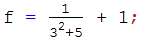
\includegraphics[width=1in]{images/scanFrac}\
\end{center}
\caption{A graphically presented declaration.} \label{fig:graphicalDecl} 
\end{figure}



% presentations are textual, or graphical (call it structural). Cannot edit this one. children can be

Because of the complexity of parsing a structural presentation and defining a meaningful subset of edit operations, Proxima disallows editing on structural presentations. Any parsing subpresentations (such as the numerator and denominator in the fraction), however, are editable again. Hence, in Figure~\ref{fig:graphicalDecl} we can type \p{+1} next to the \p{1} in the numerator, but we cannot delete the horizontal line.

After the presentation of a document has been edited, the modified presentation needs to be parsed to get an unpdate on the document structure. However, due to the mix of structural and parsing presentations, traditional parsing methods cannot readily be used. In this paper, we present the way the scanner and parser layers of Proxima co-operate in scanning and parsing graphical presentations. 

Figure~\ref{fig:scanResult} shows the result of the Proxima scanner when it is applied to the presentation in Figure~\ref{fig:scanFrac}. It consists of a nested structure of \p{ParsingTk} tokens and \p{StructuralTk} tokens. Textual tokens are represented by \p{UserTk} tokens. Each token has a subscript that denotes its unique {\em presentation identity} number. Compared to parsing tokens, structural tokens have an extra child, which is the document subtree from which it is the presentation. The document subtree is necessary since sometimes a structural presentation does not contain enough information to reconstruct the document tree.

Together with the tokens, the scanner produces a {\em whitespace map}, which is a mapping between a token's presentation identity number and its trailing whitespace. Each tuple encodes the number of trailing linebreaks and the number of trailing spaces. \todo{mention this is no good for spaces followed by linebreaks?}


\begin{figure}
\begin{footnotesize}
\begin{center}
\begin{tabbedCode}
ParsingTk$_0$ \= \\
~~ \= [ UserTk$_1$ (IdentToken "x") \\
   \> , UserTk$_2$ (OpToken "=") \\
   \> , StructuralTk$_3$ (DivExp (IntExp 1) (PlusExp ...))\\
   \> ~~~~ \= [ ParsingTk$_4$ [ UserTk$_5$ (IntToken 1)] \\
   \>      \> , ParsingTk$_6$ \= [ StructuralTk$_7$ (PowerExp (IntExp 3) (IntExp 2))\\
   \>      \>              \> ~~~~ \= [ ParsingTk$_8$    \= [ UserTk$_9$ \= (IntToken 3) ] \\
   \>      \>              \>      \> , ParsingTk$_{10}$ \> [ UserTk$_{11}$  \> (IntToken 2) ] \\
   \>      \>              \>      \> ] \\
   \>      \>              \> , UserTk$_{12}$ (OpToken "+") \\
   \>      \>              \> , UserTk$_{13}$ (IntToken 5) \\
   \>      \>              \> ] \\
   \>      \> ] \\
   \> , UserTk$_{14}$ (OpToken "+") \\
   \> , UserTk$_{15}$ (IntToken 1) \\
   \> , UserTk$_{16}$ (SymToken ";") \\
   \> ] \\
\end{tabbedCode}
\end{center}
{\bf whitespace map:} $[ 0 \mapsto (0,1), 1 \mapsto (0,1), 2 \mapsto (0,1), 9 \mapsto (0,1), 10 \mapsto (1,0) ]$
\end{footnotesize}
\caption{A scanned declaration.} \label{fig:scanResult} 
\end{figure}

%\todo{explain that all tokens in a parsingTk contain refs to their originating nonterminal in the document?}
% In case of incomplete presentation, we reuse the fields from that node. Fragile. Copy/paste, retyping, it may get lost. So only for non-essential things. 

Parsing the token structure in Figure~\ref{fig:scanResult} is relatively straightforward. For the parsing parts, we use combinator parser that has a special primitive for structural tokens. For each parsing presentation, the presentation sheet specifies the corresponding parser. The structural parts, on the other hand contain enough information to be parsed without the need to specify a parser.

The paper is organized as follows. We start by providing a brief overview of Proxima's architecture (Section~\ref{sect:architecture}) and the kind of document types that can be defined (Section~\ref{sect:documentStructure}). Then we explain the components and data types involved in presenting a document in Section~\ref{sect:presentationProcess}. The Proxima scanning and parsing algorithms are explained in sections~\ref{sect:scanner} and~\ref{sect:parser}, which form the core technical content of this paper. Section~\ref{sect:relatedWork} describes related work, and Section~\ref{sect:conclusion} concludes.






%%%%%%%%%%%%%%%%%%%%%%%%%%%%%%%%%%%%%%%%%%%%%%%%%%%%
%
\section{Proxima's layered architecture} \label{sect:architecture}
%
%%%%%%%%%%%%%%%%%%%%%%%%%%%%%%%%%%%%%%%%%%%%%%%%%%%%

The core architecture of Proxima consists of a number of layers, each communicating only with its direct neighbors. The layered structure is based on the staged nature of the presentation process and its inverse, the interpretation process.

The positions at which the document, the rendering, and the intermediate data structures reside are called {\em levels}. Between each pair of levels we have a {\em layer} that maintains the mappings between the levels. Each layer consists of a presentation component and an interpretation component. Figure~\ref{fig:levelsAndLayers} schematically shows the levels and layers of Proxima. 

\begin{figure}[ht]
\centering
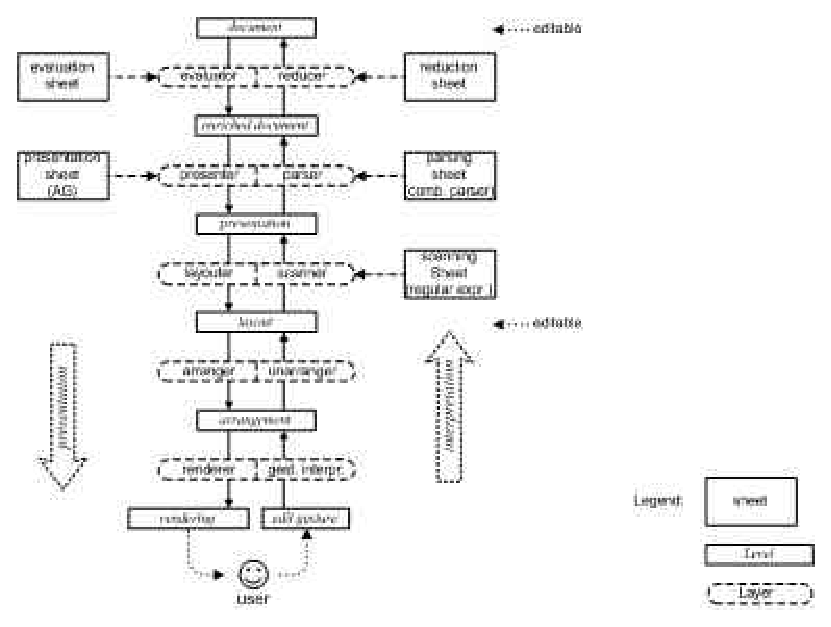
\includegraphics[width=7cm]{images/LayerOverview}
\caption{The levels and Layers of Proxima.}
\label{fig:levelsAndLayers}
\end{figure}

A data level in Proxima is not just an intermediate value in the presentation computation, but an entity in its own right. Together, the data levels constitute the state of the editor. The six data levels of Proxima are:


\begin{description}
\item[Document:] The document structure.

\item[Enriched Document:] The document enriched with derived values and structures, such as a type of a function or a table of contents, typically computed by an attribute grammar~\cite{reps84synGen}.

\item[Presentation:] A logical description of the presentation of the document, consisting of rows and columns of presentation elements with attributes. The presentation also supports formatting based on available space (e.g.\ line/page breaking).

\item[Layout:]  Presentation with explicit whitespace.

\item[Arrangement:] Formatted presentation with absolute size and position information.

\item[Rendering:] A collection of user interface commands for drawing the absolutely positioned and sized arrangement.
\end{description}

We briefly discuss each of the five layers.

\head{Evaluation layer}\\
The evaluation layer takes care of computing derived structures and values over the document, and of mapping updates on these derived structures back to document updates. In this layer, for example, type inferencing takes place. The layer is parameterized by an {\em evaluation sheet} and a {\em reduction sheet}, which specify the mappings. 

\head{Presentation layer}\\
The presentation layer consists of the presenter and the parser. The presenter takes an enriched document tree, and computes a presentation for it according to the {\em presentation sheet}. Its counterpart, the parser, maps a presentation tree back to an enriched document and is parameterized by a {\em parsing sheet}.

\head{Layout layer}\\
The layout layer handles automatic whitespace, which is maintained in the whitespace map that is part of the presentation level. For each token, the layout component looks up the corresponding whitespace and inserts actual line breaks and spaces in the presentation. The scanner recognizes tokens in the layout level, based on regular expressions specified in the {\em scanner sheet}. It also stores whitespace in the whitespace map. Because mapping tokens to strings is straightforward, the layout component does not need sheet parameter.

\head{Arrangement layer}\\
In the presentation direction, the arrangement layer computes the precise position and size for each element in the layout level. It also handles line breaking. In the interpretation direction, the only thing that needs to be done is to map absolute coordinates in edit commands to positions in the presentation tree. The arrangement level is not editable, so it need not be mapped back onto the layout level.

\head{Rendering layer}\\
The renderer creates a bitmap for the arrangement. In the other direction is the gesture interpreter, which maps edit gestures onto edit operations designated for the higher layers.

%\bl
%\o implementation: layer combinators.
%\o sometimes awkward, because we have to conform to the layers.
%\o but this has advantages: new GUI lib in a matter of days.
%\el

The two levels at which edit operations can have an effect are the document level and the layout level. After an edit operation on the document, all levels from document to rendering are updated to reflect the update. After an edit operation on the layout level, the modified layout is scanned, parsed and reduced, to obtain the corresponding updated document, from which an updated rendering is computed.

In this paper, we will focus mainly on the presentation layer and layout layer, and, more specifically, on the scanner and parser in these layers. Because we do not refer to the evaluation layer, we will use the term document to refer to the enriched document.




%%%%%%%%%%%%%%%%%%%%%%%%%%%%%%%%%%%%%%%%%%%%%%%%%%%%
%
\section{The document structure}\label{sect:documentStructure}
%
%%%%%%%%%%%%%%%%%%%%%%%%%%%%%%%%%%%%%%%%%%%%%%%%%%%%

The document type in Proxima is a monomorphic (i.e.\ parameter free) Haskell data type with lists. Below is the definition for a type \p{Decl} that represent declarations of simple expressions. 

\begin{footnotesize}
\begin{verbatim}
data Decl = Decl ident:Identifier exp:Exp {idP0,idp1}

data Identifier = Ident str:String        {idP0}

data Exp = PlusExp  exp1:Exp exp2:Exp     {idP0}
         | DivExp   exp1:Exp exp2:Exp     {idP0}
         | PowerExp exp1:Exp exp2:Exp     {idP0}
         | IntExp   val:Int               {idP0}
\end{verbatim}
\end{footnotesize}

The difference with Haskell syntax is that named fields are specified by putting an identifier and a colon in front of a child type. Furthermore, at the right of each constructor there is a number of presentation identity fields, which are used to keep track of the tokens used in the presentation. A future version of Proxima will allow presentation identities to be specified in the presentation sheet rather than the document type.

If we disregard the presentation identities, the declaration in Figure~\ref{fig:scanFrac} is represented by the following value: (the full version is provided in Section~\ref{sect:parseExample})

\begin{footnotesize}
\begin{tabbedCode}
Decl (Identifier "x")\\ 
     (PlusExp (DivExp (IntExp 1) \\
                      (PlusExp (PowerExp (IntExp 3) (IntExp 2))\\
                               (IntExp 5)))\\
              (IntExp 1))\\
\end{tabbedCode}
\end{footnotesize}


Two special constructors are added to each type by Proxima: a {\em hole} and a {\em parse error} constructor. The hole constructors make it possible to represent incomplete document trees during structural editing. The parse error constructors are used to represent a document tree that has parse errors in its presentation.





%%%%%%%%%%%%%%%%%%%%%%%%%%%%%%%%%%%%%%%%%%%%%%%%%%%%
%
\section{The presentation process}\label{sect:presentationProcess}
%
%%%%%%%%%%%%%%%%%%%%%%%%%%%%%%%%%%%%%%%%%%%%%%%%%%%%

Before discussing the scanner and parser components, we briefly discuss their counterparts in the presentation direction: the presenter and layout components. The presenter component maps an (enriched) document onto the presentation level, according to rules in the presentation sheet, which is specified with an attribute grammar. The presentation itself is a value of type \p{Xprez}, computed in a compositional way, using the\ \p{Xprez} combinator language. After the presentation phase, the presentation level is mapped onto the layout level by the layout component. In the next three subsections, we introduce the language \Xprez, the attribute grammar formalism used in the presentation sheet, and the layout component.

\subsection{The {\Xprez} presentation language} \label{sect:xprez}

\Xprez\ is a combinator library for specifying graphical presentations with support for alignment and stretching. For this paper, a short overview of the language suffices. A more complete description can be found in~\cite{schrage04Proxima}.

\begin{figure}
\begin{footnotesize}
\begin{center}
\begin{footnotesize}
\begin{verbatim}
empty             :: Xprez
text              :: String -> Xprez             
circle            :: Xprez                       
img               :: String -> Xprez             
poly              :: [(Float, Float)] -> Xprez 
row, col, overlay :: [Xprez]        -> Xprez          
rowR, colR        :: Int -> [Xprez] -> Xprez   
format            :: [Xprez]        -> Xprez
\end{verbatim}
\end{footnotesize}
\caption{The {\Xprez} primitives.} \label{fig:xprezPrim} 
\end{center}
\end{footnotesize}
\end{figure}

Figure~\ref{fig:xprezPrim} contains the \Xprez\ primitives. The basic building blocks of \Xprez\ are strings (\p{text}), tokens (\p{token}) and graphical elements such as polygons, circles, and images (\p{poly}, \p{circle}, \p{img}). With the combinators \p{row} and \p{col} presentations can be combined into rows and columns. The elements of a row or column are aligned along horizontal and vertical reference lines of their children, and do not overlap. If presentations need to overlap (for example in order to put a squiggly line under a string just below the baseline), the \p{overlay} combinator can be used. The \p{format} combinator produces a flow layout, creating rows for its children, based on available horizontal space.

Each presentation has a number of presentation attributes (e.g.\ color, font size, reference lines) that influence its appearance. Several functions are available for modifying presentation attributes. For example, for changing the font size, we can use \p{withFontsize :: Int -> Xprez -> Xprez}. \todo{mention \p{with}?}

Below is some sample \Xprez\ code that creates a graphical presentation of a fraction:

\begin{footnotesize}
\begin{verbatim}
frac e1 e2 = let numerator   = hAlignCenter (pad (shrink e1) )
                 denominator = hAlignCenter (pad (shrink e2) )
             in  colR 2 [ numerator, vSpace 2, hLine
                        , vSpace 2, denominator ] `withHStretch` False
                        
pad xp = row [ hSpace 2, xp, hSpace 2 ]

shrink e = e `withFontSize_` (\fs -> (70 `percent` fs) `max` 10)
\end{verbatim}
\end{footnotesize}

The non-primitive library function \p{hAlignCenter} centers its argument horizontally. For shrinking presentations, we use the combinator \p{withFontSize\_ :: (Int -> Int) -> Xprez -> Xprez}, which, instead of an integer, takes a function argument that computes the new font size, given its previous value.

The result of \p{frac (text "1") (text "1+x")} is~~\framebox{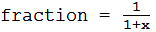
\includegraphics[width=0.5cm]{images/fracExample}}\todo{move up a bit}

Besides the combinators that produce presentations, \Xprez\ also has combinators for specifying edit operations in context menus, reactions to mouse clicks, and keeping track of document locations in the presentation.


\subsection{Document presentation}

For the presentation of the document, as well as for the computation of derived values and structures, Proxima uses the attribute grammar formalism. The presentation sheet is a file with an attribute grammar definition, which is compiled to a Haskell program by the Utrecht University AG compiler~\cite{swierstra08ag}.

For each type of node in the document, the presentation sheet defines a synthesized attribute \p{pres} of type \p{Presentation}.\todo{explain params?} In the rule for \p{pres}, the presentations of the children can be used. Besides the presentation, any number of synthesized and inherited attributes can be defined on the document tree. In this way we can easily add static checks or for example computate all variables in scope at a certain document location. Moreover, external Haskell modules can be called, allowing for complex computations, such as type checking.

% also possible edit operations specific to the doc node.

A presentation may be either {\em structural} or {\em parsing}, with the difference that parsing presentations may be edited at the presentation level whereas structural presentation may not (although they may have parsing descendents that will be editable). 

A parsing presentation consists of a sequence of tokens, which may be strings or structural presentations. In the presentation sheet, the top-most element of the parsing presentation (the one that is an immediate child of a structural presentation) must specify a parser. This parser is applied to the sequence after it has been edited.

Since a structural presentation may not be edited at the presentation level\todo{actually this is layout level}, it is straightforward to map a structural presentation back onto the document level, even if it has a graphical presentation. Hence, no parser needs to be specified in the presentation sheet.

Figure~\ref{fig:presentationSheet}\todo{add structural example without id (slide?)} shows two presentation rules for the type \p{Exp} from Section~\ref{sect:documentStructure}. The tokens are placed in a list with the \p{stream} combinator, which may also contain other token streams. The Haskell type system enforces that a parsing presentation consists only of streams and tokens. Two functions are available for creating tokens: \p{token} and \p{structuralToken}. The first parameter of both functions is a presentation identity, which is one of the p{idP} fields that is declared in the document type. The function \p{frac} in the rule for \p{DivExp} is the function that was defined in the previous subsection.

\bl
\o update
\o don't show ident power
\el

\begin{figure}
\begin{center}
\begin{footnotesize}
\begin{verbatim}
SEM Decl
  | Decl loc.pres = parsing $ stream $ [ @ident.pres, key @idP0 "="
                                       , @exp.pres,   symb @idP1 ";" ]

SEM Exp
  | PlusExp loc.pres = parsing $ stream $ [ @exp1.pres
                                          , operator @idP0 "+"
                                          , @exp2.pres ]
  | DivExp
      loc.pres = parsing $ structuralToken @idP0 $ 
                             frac @exp1.pres @exp2.pres
                  
key      idp str = token idp str `withColor` blue
operator idp str = token idp str `withColor` green
sym      idp str = token idp str `withColor` orange
\end{verbatim}
\end{footnotesize}
\caption{Presentation sheet fragment.} \label{fig:presentationSheet} 
\end{center}
\end{figure}

To every presentation rule certain extra functionality is added implicitly, e.g.\ to manage displaying the focus and to keep track of the locations in the presentation tree. Such functionality could have been supplied explicitly in the presentation sheet, but doing so is laborious and error prone. Hence, the presentation sheet contains definitions of local attributes \p{pres} rather than synthesized attributes. Automatically generated rules for the synthesized \p{pres} attributes add the default functionality to the the local attribute.


\subsection{Document layout}

The main function of the scanner is to restore the implicit whitespace and presentation focus that was recorded for each token in a parsing presentation. The  and the numberWhitespace is restored by looking up the token's whitespace in a white space map, which is kept at the presentation level, and inserting extra rows in the presentation for recorded linebreaks and strings of spaces for recorded spaces. 

Besides the whitespace, also the presentation focus is stored in the whitespace map. This is necessary because parsing and presenting a presentation does not necessarily return the same presentation. After parsing, document structures represented by tokens may be presented graphically, and then give rise to a restructured presentation. The Helium editor, for example, has a special token $\%$ that creates a graphically presented fraction. The focus restoration mechanism takes care tha after parsing and presenting the presentation focus remains at the same position. If the presentation focus cannot be restored from the tokens, the scanner will restore it by using its absolute coordinates in the presentation. 

The layout component is not parameterized by a sheet. The reason is that although we need a specification in order to create tokens from a string, the reverse process is quite easy since each token contains its string representation.  





%%%%%%%%%%%%%%%%%%%%%%%%%%%%%%%%%%%%%%%%%%%%%%%%%%%%
%
\section{Scanning}\label{sect:scanner}
%
%%%%%%%%%%%%%%%%%%%%%%%%%%%%%%%%%%%%%%%%%%%%%%%%%%%%

The function of the scanner is to map character sequences to tokens, as specified by the user in the scanner sheet. Besides this, the scanner also performs several other functions. Any structural presentation that appears in the stream of tokens is recursively scanned and recorded by a special token.

\subsection{The \p{Token} type}

Figure~\ref{fig:tokenType} shows a simplified version of the \p{Token} data type. A number of type parameters that are not important for this discussion are left out, as well as the constructors that have to do with Proxima's support for graph presentations. 

\begin{figure}
\begin{center}
\begin{footnotesize}
\begin{verbatim}
data Token Location userToken 
  = ParsingTk    IDP Location (Parser userToken) [Token node userToken]
  | StructuralTk IDP Location                    [Token node userToken]
  | UserTk       IDP userToken String 
  | ErrorTk      IDP String 
\end{verbatim}
\end{footnotesize}
\caption{The \p{Token} data type.} \label{fig:tokenType} 
\end{center}
\end{figure}

% Position is not shown ID has enough information
% Location

Each constructor has an \p{IDP} field that is used to associate the token with whitespace and focus information, which is stored in a separate map. All tokens except \p{ErrorTk} have a \p{Location} field that refers to the node in the document tree from which the token originated. (Because \p{ErrorTk} tokens originate from the scanner they do not have this field.) the \p{Location} field is used when parsing structural presentations (which is explained in Section~\ref{subsect:parsingStructural}.)

\begin{description}
\item[\p{ParsingTk}:] Represents a parsing presentation. The field \p{Parser userToken} is the parser that is used to parse the child tokens. The list of tokens will not contain any \p{ParsingTk} tokens. Instead, tokens from all parsing descendents are collected and placed in the same list. \\
\item[\p{StructuralTk}:] Represents a structural presentation and has a list of tokens for its child presentations. The \p{Location} argument is also used to access the values of children that are not presented. 
%\todo{Presentation arg has been removed, structurals are assumed not to have parse errors}
\item[\p{UserTk}:] Represents a string token. %\todo{Also has Location, not shown here} \\
\item[\p{ErrorTk}:] This constructor is used to represent lexical errors. Section~\ref{sect:parseScanErrors} explains its use. \\
\end{description}




\subsection{The scanner sheet}

The lexical analysis of textual tokens is based on the Haskell lexical analyser generator Alex~\cite{marlow07alex}. Alex is a tool that generates an efficient lexical analyser based on a description of the tokens in the form of regular expressions. It is comparable to the lex and flex tools for C and C++.

An editor designer has to define the data type \p{UserToken} and provide an Alex specification for the tokens. Figure~\ref{fig:scannerSheet} shows an example \p{UserToken} and scanner sheet. The Alex specification consists of a a number of macro definitions followed by a set of rules, each defining a token. A rule is a regular expression together with an action that constructs the token.

\begin{figure}
\begin{center}
\begin{footnotesize}
\begin{verbatim}
data UserToken =
       IdentToken String | OpToken String | SymToken Char | IntToken Int

$lower = [a-z]
$upper = [A-Z]
$alpha = [$lower $upper]
$digit = 0-9		
$opChar = [\+ \- \=]
$symChar = [\;]
tokens :-
 $digit+                       { mkToken $ \s   -> IntToken (read s) }
 $opChar+                      { mkToken $ \s   -> OpToken s         }
 $symChar                      { mkToken $ \[c] -> SymToken c        }
 $lower [$alpha $digit \_ \']* { mkToken $ \s   -> IdentToken s      }
\end{verbatim}
\end{footnotesize}
\caption{Example \p{UserToken} and scanner sheet.} \label{fig:scannerSheet} 
\end{center}
\end{figure}

The only difference between a normal Alex description and a Proxima scanner sheet is that each action needs to be preceded by a \p{mkToken} application. The \p{mkToken} application takes care of passing the internal scanner state, and constructing a \p{UserTk} alternative of type \p{Token}. %\todo{mention it assigns IDP}



\subsection{Scanning the presentation}

The scanner traverses the layout tree and creates a tree of structural and parsing tokens that matches the structure of the presentation. \p{mention that parsing subtrees are merged} The behavior of the scanner is determined by the kind of presentation on which it is called.


% How the tokenizer works:
\head{Structural presentation} \\
A structural presentation of a document node is an Xprez tree containing presentations of child nodes. The scanner traverses the presentation tree and makes a recursive call on each child presentation that is encountered. The list of child tokens is put in a \p{StructuralTk} and returned as the result of the scanner.

\head{Parsing presentation} \\
A parsing presentation consists of a column of rows, which contain either strings or structural presentations. Each structural presentation is mapped onto a structural token by recursively scanning it. The sequences of strings between the structural tokens are first extended with newline characters to mark the transitions between rows. The resulting lists of characters are mapped onto lists of \p{UserTk} tokens by applying the Alex scanner. The final list of child tokens is the result of merging the structural tokens with the recognized user tokens.


\subsection{Handling whitespace}

% Whitespace
In order to use the automatic whitespace recognition, the following rule must be added to scanner sheet:

\begin{footnotesize}
\begin{verbatim}
  [\n \ ]+        { collectWhitespace }
\end{verbatim} %$
\end{footnotesize}

As a result, the scanner emits special tokens for sequences of whitespace. A post processing phase removes these whitespace tokens, and records the trailing whitespace for each token in the whitespace map. \todo{say more about focus?}

\bl
\o leading whitespace is added to first token. If non empty, then always be a first token, or a parse error, which takes care. So expression no problem. however list of decl, extra IDP field and on top-level parser variant of parsing that records the idp.
\el

\bl
\o rather simple model breaks spaces. More liberal is spaces between linebreaks. Also comments. Easy to 
\el
% first token whitespace








%%%%%%%%%%%%%%%%%%%%%%%%%%%%%%%%%%%%%%%%%%%%%%%%%%%%
%
\section{Parsing}\label{sect:parser}
%
%%%%%%%%%%%%%%%%%%%%%%%%%%%%%%%%%%%%%%%%%%%%%%%%%%%%

Unlike ordinary parsers, which take a list of tokens to produce a value, the Proxima parser is a function that takes only one token as input. This token can be either a structural token or a parsing token. In case of a structural token, the value is constructed automatically from the list of child tokens. If the token is a parsing token, its list of children is fed into the parser that was specified in the presentation sheet.

\subsection{Structural presentations}\label{subsect:parsingStructural}

A structural token corresponds to the presentation of a certain document node and contains a list of tokens that correspond to child-presentations that were part of the presentation of that document node. Each child may be presented multiple times, or even not at all. Furthermore, the order in which the child presentations appear may not correspond to the order of the children in their parent node.

Nevertheless, we can parse a structural token automatically, since all tokens contain a \p{Location} reference to the document node and path from which they were presented. Hence, we can deduce for each token for which child of the document node it is a presentation. Because structural presentations are not edited at the presentation level, this information will still be valid after the presentation has been edited. 

For child$_i$ of the document node, the parser takes the list of tokens that contain presentations of that child. If this list is empty, the presentation does not contain a presentation for the child, and we use its previous value, which is stored in the structural token. If the list is not empty, the token for the presentation that was edited is selected and this is recursively parsed to yield a value for child$_i$. In case no presentation was edited, the child value is also reused from the structural token, for efficiency. There will be at most one edited presentation, since Proxima does not allow editing multiple presentations for a single value at the same time. \todo{check is not enforced yet}

\todo{untyped, but safe}



\subsection{Parsing presentations}

The parser for a parsing presentation cannot be constructed automatically from the presentation. Instead, we use the parser that was specified in the presentation sheet, which is stored in the \p{ParsingTk} value. These parsers are specified using the UU Parsing library~\cite{swierstra03polishParsers, swierstra08parserCombinators}. This is a library for creating fast error correcting parsers with support for user-friendly error messages. Because of the error recovery, parsing does not stop after the first error, and hence multiple parse errors in different parts of the presentaiton can be reported. \todo{The fact that they always produce a result is not used}

A Proxima parser is very similar to a regular parser specified with a combinator parser library. The only difference is that, in order to let the scanner handle whitespace and focus restoration, the presentation id's of the parsed tokens need to be stored in the appropriate fields of the document node. 

The list of tokens to which the parser is applied will all be either \p{UserTk}, \p{StructuralTk}, or \p{ErrorTk} tokens, since nested \p{ParsingTk} tokens are not created by the scanner. Primitive parsers are available for user tokens and structural tokens. No primitive parser is offered for error tokens, since these signal a lexical error by the scanner, which should always lead to a parse error.

In line with the previous examples, we show part of a parser for expressions. The parser does not take into account priorities.\todo{mention that holes need to be explicitly parsed?}

%%%%%%%%%% max verbatim width, footnotesize %%%%%%%%%%%%%%%%%%%%%%%%%%%%
\begin{footnotesize}
\begin{verbatim}
parseDecl :: Parser Decl
parseDecl = 
      (\id eqTk exp semiTk-> Decl (getIDP eqTk) (getIDP semiTk) id exp)
  <$> parseIdent <*> pToken (KeyToken "=") 
  <*> parseExp <*> pToken (SymToken ';')
       
parseExp :: Parser Exp
parseExp = (\tk e1 e2 -> PlusExp (getIDP tk) e1 e2)
       <$> pToken (OpToken "+") <*> parseExp <*> parseExp
   <|> pStructural Node_Div
   <|> pStructural Node_Power
\end{verbatim}
\end{footnotesize}
\bl
\o check
\el

The \p{pToken} parser is a primitive parser that succeeds on the \p{UserToken} value that is passed as an argument. The \p{pStructural} parser succeeds on a structural token for a value of the type that is denoted with its argument. The argument is of type \p{Token} which is a generated union of all constructors in the document.\todo{not the type, but the constructor} 

Although Proxima currently uses the UU Parsing library, this connection is not fixed. In fact, any  parser library that allows a user-defined token type as input and produces Haskell values is suitable. Hence, a binding with for example the Parsec library~\cite{leijen08parsec} is also possible. The only thing that needs to be done in order to use a different library is to define a primitive parser \p{pStructural}.

\subsection{Example} \label{sect:parseExample}

As an example of the parser, we show the result of parsing the tokens in Figure~\ref{fig:scanExample} that were obtained from scanning: 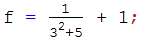
\includegraphics[width=1in]{images/scanFrac}


\begin{footnotesize}
\begin{tabbedCode}
Decl$_{2,16}$ \= (Identifier$_1$ "x")\\ 
              \> (PlusExp$_{14}$ \= (DivExp$_3$ \= (IntExp$_5$ 1) \\
              \>                 \>             \> (PlusExp$_{12}$ \= (PowerExp$_7$ (IntExp$_9$ 3) (IntExp$_{11}$ 2))\\
              \>                 \>             \>                 \> (IntExp$_{13}$ 5)))\\
              \>                 \>(IntExp$_{15}$ 1))\\
\end{tabbedCode}
\end{footnotesize}

\bl
\o same as in .... But now pres id's are shown (2 for Decl.) Correspond to token id's
\o Pres id's for parsing token are not here. Because empty is error. Ref to section..
\el

\subsection{Parse errors} \label{sect:parseScanErrors}

On a parse error, a parser does not return a document tree, which means there will not be a document to present. To account for this, the parser can return a special parse error value, for which a constructor is added to each type in the document. For a document type $Type$, this constructor has the following form:

\begin{footnotesize}
\begin{tabbedCode}
data $Type$ =
  ...
  | ParseErr\_$Type$ [ErrorMessage] [Token node userToken] 
\end{tabbedCode}
\end{footnotesize}

When a parse error is encountered, the parser constructs a \p{ParseErr} value and supplies it with a list of error messages and the list of tokens it tried to parse. The presenter uses the list of tokens when the parse error node is presented. In addition, squiggly lines are put at the presentation of tokens that are referenced in the \p{ErrorMessages} list. The whitespace for the tokens in the parse error node was already handled by scanner, and is restored by the layout component in the same way as it is for tokens from ordinary presentation.

Each type of node in the document has a generated synthesized attribute \p{parseErrors}, which is the collection of all parse errors in the nonterminal or its descendents. This attribute can be used to show a list of parse errors in the presentation. 


% lexical errors
Lexical errors require a special treatment. When Alex encounters a lexical error, it stops at the offending character. The offending character and the remainder of the input are put in an \p{ErrorTk} token, which will always cause a parse error since no primitive parser is offered that accepts it. Since scanning the string stops at the offending character, all following whitespace  will be recorded in the string, rather than stored in the whitespace map. The layout component, therefore, treats error tokens specially, by expanding any whitespace that is encoded in the string. %\todo{interpretation extra state in parsing will require storing ScanChars rather than chars}






%%%%%%%%%%%%%%%%%%%%%%%%%%%%%%%%%%%%%%%%%%%%%%%%%%%%
%
\section{Related work}\label{sect:relatedWork}
%
%%%%%%%%%%%%%%%%%%%%%%%%%%%%%%%%%%%%%%%%%%%%%%%%%%%%



Editors for mathematical formulas, such as AmayaMathematica~\cite{mathematica} However, these systems work for a fixed document type, which is not easily extensible. Eisenberg and Kiczales describe a presentation extension formalism for Eclipse, but their solution is based on the Java language.

The Barista~\cite{KoMyers06Barista} framework has similarities to Proxima, although it is targeted mainly at code editors. The system allows graphical presentations for program structures, but these are expanded to the underlying textual presentation when the user 
\bc
older systems either had text only synthesizer generator, asfsdf. Or purely structural visual redwood + some other visual langs, but then no free text editing.

Many systems such as Mathematica, or amaya do support  but only on fixed type. More flexible Eisenberg Kiczales but still for Java. 

More modern is Barista. Allows graphical views. However, when editing the view, it is expanded to its sequential representation. Good as an option, but in many cases unnecessary. 



\noindent Barista~\cite{KoMyers06Barista} is a powerful framework for building code editors. It is built on top of Citrus~\cite{KoMyers05Citrus}, which is a UI toolkit together with an object-oriented language. Although Barista is targeted at code editors, the presentation of the code can be visual, for example allowing for images to appear in comments, or having graphical presentations of code. The editors created with Barista are syntax directed, but presentation-oriented editing is available. 

\ec



%%%%%%%%%%%%%%%%%%%%%%%%%%%%%%%%%%%%%%%%%%%%%%%%%%%%
%
\section{Conclusion}\label{sect:conclusion}
%
%%%%%%%%%%%%%%%%%%%%%%%%%%%%%%%%%%%%%%%%%%%%%%%%%%%%


Editors for programming languages can benefit from offering editable graphical presentations of programs. Such graphical presentations, however, cannot be parsed with conventional parsing techniques. In this paper, we introduced a method for scanning and parsing graphical presentations.  A combinator parser is used for textual parts of the presentations, whereas the graphical parts are recognized automatically, based on information in the presentation itself.

The scanner and parser are part of the Proxima generic editor, and have been used to implement a number of prototype editors.
\bc
The Proxima system is still under development. No special attention to incrementality. Current parsers are fast. In a background thread. Scanner also not incremental, although quite easy to realize. Tests will have to show if this is nec.

The parsing method described in this paper allows for easy construction Allows editors to finally let go of ascii and provide a rich view ...
\ec
\bc
\bl
\o document extra state in parsing presentations not shown here.
\el

\bl
\o comments can be handled similar to whitespace and focus
\o more static checks are possible
\o easy ways to increase speed after change management
\o Proxima allows building IDE with only little effort.
\o use ag to add static/type checks
\el
\ec


%%%%%%%%%%%%%%%%%%%%%%%%%%%%%%%%%%%%%%%%%%%%%%%%%%%%
%
% References

\bibliographystyle{sbc}
\bibliography{../proxima}

\end{document}
